% Provenance (never printed): see sources/outline_sources.md (Year 1: decay systems K-Ar,
% Rb-Sr, U-Pb and radiocarbon; closure temperature; dating sedimentary sequences with
% volcanic ashes; calibrating the scale). Exercise and problem values in the Book 3
% scratch calculator calc/ch25.py; figures from figdata/bachelor-1/decay_curves.py,
% isochron.py and radiocarbon.py (IntCal20, dataset bachelor-1-intcal20).
% The decay law, half-life and decay constant belong to the physics series (recalled);
% the closed system and the isochron of minerals are Book 2's (g12 age-of-the-earth),
% re-founded here with whole-rock samples and least squares. The concordia diagram and
% thermochronology are the Year 3 volume's: prose pointers only. Mass spectrometry is
% the chemistry series' (recalled). The isochron figure uses an invented rhyolite so that
% the Varden granite of the problem is not solved in the course.
\chapter{Radiometric Dating Methods}\label{ch:b1:radiometric-methods}

In 2001 a team working on detrital grains of zircon from the Jack Hills of
Western Australia reported one that had crystallised
\num[uncertainty-mode=separate]{4404 \pm 8} million years ago. Later work confirmed the age of these
grains: they are the oldest known material of any kind formed on the Earth, and
they show that a \omterm{def:b1:layered-earth:layers}{crust} had formed within about 160 million years of the birth of
the Solar System. At the other end of the scale, argon ages have placed the
extinction at the end of the Cretaceous, \qty{66.00}{\Ma} ago, within
\num{32000} years of the impact thought to have caused it. Both numbers come from counting atoms: a radioactive parent that decays at a
known rate, a daughter that accumulates. This chapter explains how such clocks
are read, why each dates a different event, and how they hang the chart of
\cref{ch:b1:stratigraphic-scale} on a scale of years.
% ledger: wilde01:4404, uw14:jack-hills, ics:base.Paleogene, renne:kpg

\begin{omfigure}
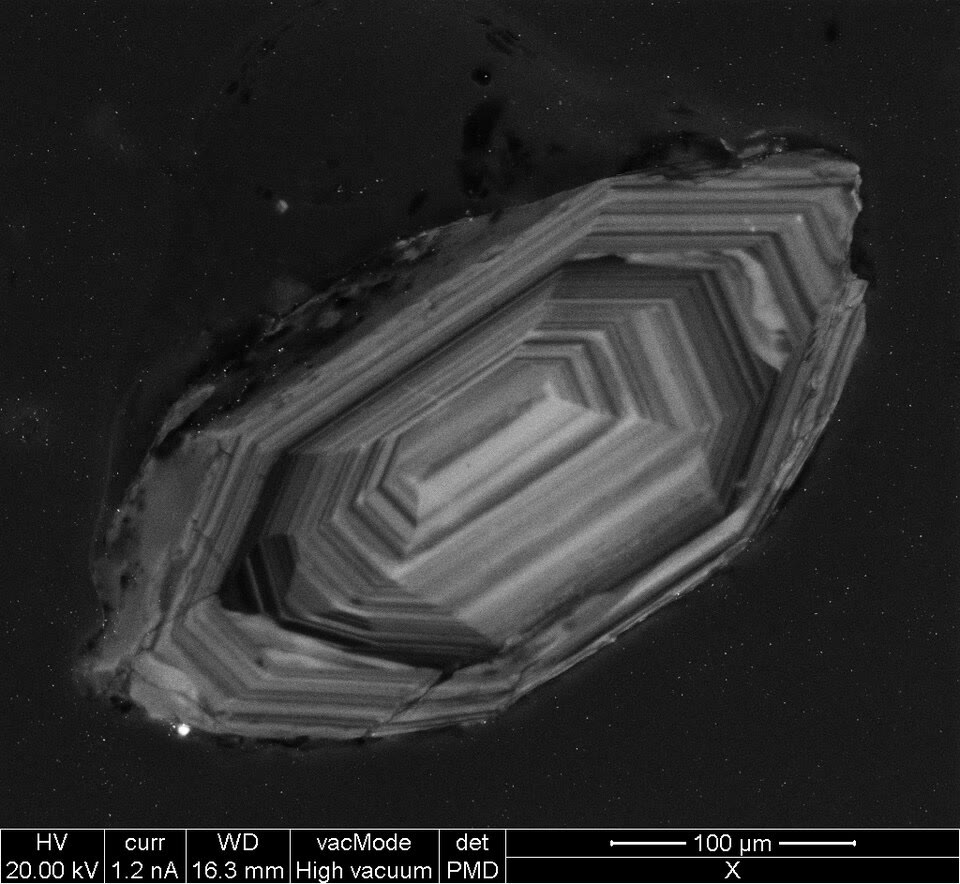
\includegraphics[width=0.5\linewidth]{images/book3/b1-zircon-cl.jpg}

{\small A grain of zircon, about a third of a millimetre long, imaged by the
light it emits under the electron beam of a scanning electron microscope
(cathodoluminescence). The bands that follow the faces of the crystal are
zones of slightly different composition, laid down one after another as it
grew. This grain was picked from a sandstone, so it is older than the sandstone:
it dates the rock it was eroded from. (Emmanuel Roquette, CC~BY-SA~4.0, via
Wikimedia Commons.)}
\label{fig:b1:radiometric-methods:zircon}
\end{omfigure}
% ledger: commons:zircon-cl

\begin{recall}
The physics volumes describe radioactive decay: the nuclei of a radioactive
isotope decay at random, independently of temperature and pressure, so that the
number $N$ left after a time $t$ follows $N = N_0\,e^{-\lambda t}$, where
$\lambda$ is the decay constant; the half-life is $T = \ln 2/\lambda$. Isotopes
of an element have the same number of protons and different numbers of
neutrons; the chemistry volumes describe the mass spectrometer, which sorts ions
by mass. In Book~2, grade~12, a rock or \omterm{def:b1:rock-forming-minerals:mineral}{mineral} that has exchanged no parent or
daughter atoms with its surroundings is a closed system, and the \omterm{def:b1:rock-forming-minerals:mineral}{minerals} of the
Varden granite, plotted on a rubidium--strontium \omterm{def:b1:radiometric-methods:isochron}{isochron}, gave an age of 310
million years. Biotite, muscovite and hornblende are the \omterm{def:b1:rock-forming-minerals:groups}{micas} and the \omterm{def:b1:rock-forming-minerals:groups}{amphibole}
of \cref{def:b1:rock-forming-minerals:groups}. An age between two dated levels
can be interpolated (\cref{prop:b1:stratigraphic-scale:interpolation}).
\end{recall}
% ledger: tulane:radiometric, villa22:rb87

\section{Decay systems}\label{sec:b1:radiometric-methods:systems}

A clock needs two counts: what is left of the parent, and how much daughter it has
made since the clock started.

\begin{definition}[Parent isotope, radiogenic daughter]\label{def:b1:radiometric-methods:radiogenic}
In a decay system used for dating, the \emph{parent isotope}\index{parent
isotope} is the radioactive isotope whose decay serves as the clock, and the
daughter is the isotope its decay produces. The \emph{radiogenic
daughter}\index{radiogenic daughter}, written $D^*$, is the part of the
daughter made by the decay of the parent inside the sample since the clock
started; the rest, $D_0$, was there from the start. The number of atoms of the
daughter measured today is $D = D_0 + D^*$.
\end{definition}

\begin{proposition}[Radiogenic growth and the age equation]\label{prop:b1:radiometric-methods:growth}
In a closed system that contains $P$ atoms of the parent today, the \omterm{def:b1:radiometric-methods:radiogenic}{radiogenic
daughter} made in a time $t$ is
\[
  D^* = P\,\bigl(e^{\lambda t} - 1\bigr),
\]
provided each decay gives one atom of the daughter. The age is then
\[
  t = \frac{1}{\lambda}\,\ln\!\left(1 + \frac{D^*}{P}\right).
\]
\end{proposition}

\begin{proof}
By the decay law the parent numbered $P_0 = P\,e^{\lambda t}$ when the clock
started. In a closed system every missing parent atom has become a daughter
atom, so $D^* = P_0 - P = P\,(e^{\lambda t} - 1)$. Then $e^{\lambda t} = 1 +
D^*/P$; taking logarithms gives the age.
\end{proof}

The age depends only on a ratio of two numbers of atoms, which is what a mass
spectrometer measures best. The figure below shows the two counts in units of
the half-life: after one half-life $D^*/P = 1$, after two $3$, after three $7$
--- in general $2^n - 1$ after $n$ half-lives.

\begin{omfigure}
\begin{tikzpicture}
\begin{axis}[omrecord, width=0.72\linewidth, height=5.6cm, xmin=0, xmax=5, ymin=0, ymax=1.05,
  xlabel={time (half-lives)}, ylabel={fraction of the initial parent},
  xtick={0,1,...,5}, ytick={0,0.25,0.5,0.75,1}]
% computed in figdata/bachelor-1/decay_curves.py (no real-world number)
\addplot[omThm, line width=1pt] table[x=n, y=P] {figdata/out/bachelor-1-decay_curves-curves.dat};
\addplot[omDef, line width=1pt] table[x=n, y=D] {figdata/out/bachelor-1-decay_curves-curves.dat};
\addplot[only marks, mark=*, mark size=1.4pt, black!60] table[x=n, y=P] {figdata/out/bachelor-1-decay_curves-marks.dat};
\addplot[only marks, mark=*, mark size=1.4pt, black!60] table[x=n, y=D] {figdata/out/bachelor-1-decay_curves-marks.dat};
\node[font=\small, text=omThm, anchor=south west] at (axis cs:0.35,0.80) {parent $P$};
\node[font=\small, text=omDef, anchor=north west] at (axis cs:2.55,0.66) {radiogenic daughter $D^*$};
\node[font=\scriptsize, anchor=west, inner sep=1pt] (r1) at (axis cs:0.12,0.5) {$D^*/P = 1$};
\draw[black!60, line width=0.4pt] (r1.east) -- (axis cs:0.95,0.5);
\node[font=\scriptsize, anchor=south] at (axis cs:2,0.77) {$3$};
\node[font=\scriptsize, anchor=south] at (axis cs:3,0.89) {$7$};
\node[font=\scriptsize, anchor=north] at (axis cs:4,0.915) {$15$};
\node[font=\scriptsize, anchor=north east] at (axis cs:4.97,0.95) {$31$};
\end{axis}
\end{tikzpicture}

{\small The parent and its \omterm{def:b1:radiometric-methods:radiogenic}{radiogenic daughter} in a closed system, as fractions of
the initial number of parent atoms, against time counted in half-lives. Their sum
stays equal to one; the ratio $D^*/P$, printed at each whole half-life, doubles
and adds one at each step.}
\label{fig:b1:radiometric-methods:decay}
\end{omfigure}

A clock reads well only within a window of ages. Long before one half-life the
daughter is a tiny fraction of the parent; after many half-lives too little
parent is left to measure. The table below lists the systems most used, with the
material each is applied to.

\begin{table}[ht]
\centering
\small
\renewcommand{\arraystretch}{1.25}
\begin{tabular}{|l|l|c|c|>{\raggedright\arraybackslash}p{4.3cm}|}
\hline
parent & daughter & half-life (years) & $\lambda$ (per year) & dated material \\
\hline
$^{14}\mathrm{C}$ & $^{14}\mathrm{N}$ & \num{5700} & \num{1.216e-4} & wood, charcoal, bone, shell \\
$^{40}\mathrm{K}$ & $^{40}\mathrm{Ar}$, $^{40}\mathrm{Ca}$ & \num{1.25e9} & \num{5.543e-10} & potassium-rich \omterm{def:b1:rock-forming-minerals:mineral}{minerals}: sanidine, biotite, hornblende \\
$^{87}\mathrm{Rb}$ & $^{87}\mathrm{Sr}$ & \num{4.96e10} & \num{1.3972e-11} & granites (whole rocks), \omterm{def:b1:rock-forming-minerals:groups}{micas} \\
$^{147}\mathrm{Sm}$ & $^{143}\mathrm{Nd}$ & \num{1.07e11} & \num{6.46e-12} & rocks and their \omterm{def:b1:rock-forming-minerals:mineral}{minerals} (\omterm{def:b1:radiometric-methods:isochron}{isochrons}) \\
$^{235}\mathrm{U}$ & $^{207}\mathrm{Pb}$ & \num{7.04e8} & \num{9.8485e-10} & zircon \\
$^{238}\mathrm{U}$ & $^{206}\mathrm{Pb}$ & \num{4.47e9} & \num{1.55125e-10} & zircon \\
\hline
\end{tabular}
\caption{The main decay systems. The decay constants of potassium-40 and of the
two uraniums are the conventional values used to compute ages; those of
rubidium-87 and samarium-147 are computed from the half-lives, that of
carbon-14 from its half-life of \num{5700} years.}
\label{tab:b1:radiometric-methods:systems}
\end{table}
% ledger: iaea:c14, iaea:k40-branches, amherst:constants, villa22:rb87, iaea:sm147, iaea:isotopes, tulane:kar, tulane:upb-zircon, tulane:c14

Two sets of numbers are in use for the same nuclei, and an age must say which
it used. Nuclear data tables give potassium-40 a half-life of
\num{1.248e9} years and send \qty{10.72}{\percent} of its decays to argon; the
constants conventionally used in geochronology give $\lambda = \num{5.543e-10}$ per year (a half-life of \num{1.2505e9}
years) and send $0.581/5.543 = \qty{10.48}{\percent}$ of the decays to argon.
\omterm{def:b1:radiometric-methods:radiocarbon}{Radiocarbon ages}, as \cref{sec:b1:radiometric-methods:kar} explains, are
computed with a half-life of \num{5568} years that is known to be too short. The
differences reach a few per cent, far more than the \qty{0.01}{\percent} to which
the best ages are now quoted (\cref{sec:b1:radiometric-methods:sediments}).
The uncertainty of the decay constants of potassium-40 itself, a nucleus with
two branches and a long half-life, limits the accuracy of its ages.
% ledger: iaea:k40-branches, amherst:constants, sp77:conventional-age, ics:base.Triassic, nmgrl:arar

\begin{proposition}[Precision of an age]\label{prop:b1:radiometric-methods:precision}
If the ratio $R = D^*/P$ is measured with the standard uncertainty $\sigma_R$,
the age carries the uncertainty
\[
  \sigma_t = \frac{\sigma_R}{\lambda\,(1 + R)}.
\]
\end{proposition}

\begin{proof}
For a small error $\delta R$, the age $t = \ln(1+R)/\lambda$ changes by
$\delta t = t'(R)\,\delta R = \delta R/\bigl(\lambda(1 + R)\bigr)$.
\end{proof}

For a young sample, $R$ is small and $\sigma_t \approx \sigma_R/\lambda$: the
absolute error of the age is set by how well a small amount of daughter can be
measured. A long half-life (small $\lambda$) magnifies it. That is why
rubidium--strontium and uranium--lead serve for rocks older than about ten
million years, while potassium--argon reaches rocks as young as about ten
thousand years, and radiocarbon covers the last \num{70000} years.
% ledger: tulane:ranges

\section{Isochrons}\label{sec:b1:radiometric-methods:isochrons}

The age equation needs $D^*$, but the instrument measures $D = D_0 + D^*$, and
$D_0$ is rarely zero: strontium-87 is present in every \omterm{def:b1:rock-forming-minerals:mineral}{mineral} that took in
strontium when it formed. The \omterm{def:b1:radiometric-methods:isochron}{isochron} removes $D_0$ by measuring several
samples that started with the same isotopic composition of the daughter element.

\begin{definition}[Isochron, initial ratio]\label{def:b1:radiometric-methods:isochron}
Let $S$ be a stable isotope of the daughter element that no decay produces
($^{86}\mathrm{Sr}$ for strontium, $^{144}\mathrm{Nd}$ for neodymium). An
\emph{isochron}\index{isochron} is the straight line on which plot, in a graph
of $y = D/S$ against $x = P/S$, samples that formed at the same time with the
same value of $D/S$ and have been closed systems since. That shared starting
value $y_0 = (D/S)_0$ is the \emph{initial ratio}\index{initial ratio}.
\end{definition}
% ledger: tulane:radiometric, tulane:c14

\begin{theorem}[The isochron]\label{thm:b1:radiometric-methods:isochron}
Samples that formed at the same time with the same \omterm{def:b1:radiometric-methods:isochron}{initial ratio} $y_0$, and have
been closed systems for a time $t$, satisfy
\[
  y = y_0 + \bigl(e^{\lambda t} - 1\bigr)\,x .
\]
Their points lie on a straight line of slope $m = e^{\lambda t} - 1$ and
intercept $y_0$, and $t = \ln(1+m)/\lambda$.
\end{theorem}

\begin{proof}
For each sample, $D = D_0 + P\,(e^{\lambda t} - 1)$ by
\cref{prop:b1:radiometric-methods:growth}. The number of atoms of $S$ has not
changed, since $S$ is stable, made by no decay, and the system is closed;
dividing by it gives $y = y_0 + (e^{\lambda t} - 1)\,x$, with $y_0$ the same for
all samples by hypothesis.
\end{proof}

When a granite crystallised, all its samples had the same $y_0$ and plotted on a
horizontal line; each has since moved up in proportion to its $x$, and the line
has turned about its intercept. The samples need different values of $x$ to
define the slope well: \omterm{def:b1:rock-forming-minerals:mineral}{minerals} with much and little rubidium, as in Book~2, or
whole-rock samples taken from more and less evolved parts of one intrusion. A
point off the line marks a sample that was not closed, or did not share the
\omterm{def:b1:radiometric-methods:isochron}{initial ratio}. The \omterm{def:b1:radiometric-methods:isochron}{initial ratio} is itself a tracer: a magma from the \omterm{def:b1:layered-earth:layers}{mantle}
inherits a low $^{87}\mathrm{Sr}/^{86}\mathrm{Sr}$, about $0.7025$, and one from
melted continental \omterm{def:b1:layered-earth:layers}{crust} a high one, about $0.710$, because the \omterm{def:b1:layered-earth:layers}{crust} is rich in
rubidium and has made more strontium-87 over the ages.
% ledger: tulane:radiometric, tulane:sr-initial

Real points never fall exactly on a line. The usual estimate of the line is the
one that makes the squared vertical distances of the points to it as small as
possible.

\begin{proposition}[The least-squares line]\label{prop:b1:radiometric-methods:lsq}
Let $(x_i, y_i)$, $i = 1, \dots, n$, be points with at least two different $x_i$,
of means $\bar x$ and $\bar y$, and let
\[
  S_{xx} = \sum_i (x_i - \bar x)^2, \qquad S_{xy} = \sum_i (x_i - \bar x)(y_i - \bar y).
\]
The line $y = b + m x$ that minimises $Q(b, m) = \sum_i (y_i - b - m x_i)^2$ has
\[
  m = \frac{S_{xy}}{S_{xx}}, \qquad b = \bar y - m\,\bar x ,
\]
and passes through the centroid $(\bar x, \bar y)$.
\end{proposition}

\begin{proof}
$Q$ is a sum of squares, a polynomial of degree two in $(b, m)$ that tends to
infinity in every direction, so it reaches its minimum where both partial
derivatives vanish. $\partial Q/\partial b = -2 \sum_i (y_i - b - m x_i) = 0$
gives $n\bar y = n b + n m \bar x$, so $b = \bar y - m \bar x$: the line passes
through the centroid. Substituting, $y_i - b - m x_i = (y_i - \bar y) - m(x_i -
\bar x)$, and $\partial Q/\partial m = -2 \sum_i x_i \bigl[(y_i - \bar y) - m(x_i
- \bar x)\bigr] = 0$. Since $\sum_i (y_i - \bar y) = \sum_i (x_i - \bar x) = 0$, $x_i$
may be replaced by $x_i - \bar x$ in this sum, which gives $S_{xy} - m S_{xx} = 0$.
$S_{xx} > 0$ because the $x_i$ are not all equal.
\end{proof}

The scatter of the points about the line gives the uncertainty of the slope.
With the residuals $r_i = y_i - b - m x_i$, the standard deviation of the
scatter is $s = \sqrt{\sum_i r_i^2/(n-2)}$ --- two degrees of freedom are used
by the two parameters --- and the standard uncertainties of the slope and of the
intercept are
\[
  \sigma_m = \frac{s}{\sqrt{S_{xx}}}, \qquad
  \sigma_b = s\,\sqrt{\frac1n + \frac{\bar x^2}{S_{xx}}} .
\]
These two results of statistics are admitted here; the age then carries
$\sigma_t = \sigma_m/\bigl(\lambda(1 + m)\bigr)$, by the argument of
\cref{prop:b1:radiometric-methods:precision}. They show what makes a good
\omterm{def:b1:radiometric-methods:isochron}{isochron}: many points, spread widely in $x$ (a large $S_{xx}$), with little
scatter.

\begin{method}[Fitting an isochron]\label{met:b1:radiometric-methods:isochron}
\begin{enumerate}
  \item Measure $x = P/S$ and $y = D/S$ in at least four samples of one body,
        chosen to spread $x$ as widely as possible.
  \item Plot them; set aside, with a reason, any point clearly off the trend.
  \item Compute $\bar x$, $\bar y$, $S_{xx}$, $S_{xy}$, then $m = S_{xy}/S_{xx}$
        and $b = \bar y - m \bar x$.
  \item Compute the residuals, $s$, $\sigma_m$ and $\sigma_b$.
  \item The age is $t = \ln(1+m)/\lambda$, with $\sigma_t =
        \sigma_m/\bigl(\lambda(1+m)\bigr)$; the \omterm{def:b1:radiometric-methods:isochron}{initial ratio} is $b \pm \sigma_b$.
\end{enumerate}
\end{method}

\begin{example}[An invented rhyolite]\label{ex:b1:radiometric-methods:rhyolite}
Six whole-rock samples of a series of rhyolite lavas (exercise data) give:
\begin{center}
\small
\begin{tabular}{|l|cccccc|}
\hline
$x = {}^{87}\mathrm{Rb}/^{86}\mathrm{Sr}$ & 1.85 & 4.62 & 9.30 & 14.75 & 21.20 & 27.60 \\
$y = {}^{87}\mathrm{Sr}/^{86}\mathrm{Sr}$ & 0.71732 & 0.73332 & 0.76164 & 0.79420 & 0.83226 & 0.87028 \\
\hline
\end{tabular}
\end{center}
Here $\bar x = 13.22$, $\bar y = 0.784837$, $S_{xx} = 491.41$ and
$S_{xy} = 2.92308$, so $m = 0.0059484$ and $b = 0.70620$. The residuals give
$s = 0.00024$, $\sigma_m = \num{1.10e-5}$ and $\sigma_b = 0.00018$. The age is
$t = \ln(1.0059484)/\num{1.3972e-11} = \qty{424.5}{\Ma}$, with
$\sigma_t = \num{1.10e-5}/(\num{1.3972e-11} \times 1.0059) = \qty{0.8}{\Myr}$:
\qty[uncertainty-mode=separate]{424.5(8)}{\Ma}, \omterm{def:b1:radiometric-methods:isochron}{initial ratio}
\num[uncertainty-mode=separate]{0.70620(18)} (figure below).
\end{example}
% values: isochron.py (slope 0.005948361, intercept 0.7061993, age 424.4732, sigma 0.7827871); ledger: villa22:rb87

\begin{omfigure}
\begin{tikzpicture}
\begin{axis}[omrecord, width=0.74\linewidth, height=6cm, xmin=0, xmax=30, ymin=0.70, ymax=0.88,
  xlabel={$^{87}\mathrm{Rb}/^{86}\mathrm{Sr}$}, ylabel={$^{87}\mathrm{Sr}/^{86}\mathrm{Sr}$},
  ytick={0.70,0.72,...,0.88},
  y tick label style={/pgf/number format/.cd, fixed, fixed zerofill, precision=2}]
% computed in figdata/bachelor-1/isochron.py (exercise data, invented rhyolite); ledger: villa22:rb87
\addplot[black!60, densely dotted, line width=0.7pt] table[x=x, y=y] {figdata/out/bachelor-1-isochron-initial.dat};
\addplot[omDef, line width=0.9pt] table[x=x, y=y] {figdata/out/bachelor-1-isochron-line.dat};
\addplot[omThm, only marks, mark=*, mark size=2pt] table[x=x, y=y] {figdata/out/bachelor-1-isochron-points.dat};
\node[font=\scriptsize, text=omDef, anchor=south east, align=right] at (axis cs:19,0.83)
  {least-squares slope $0.005948$\\ age \qty[uncertainty-mode=separate]{424.5(8)}{\Ma}};
\node[font=\scriptsize, text=black!70, anchor=south west] at (axis cs:9,0.7068)
  {initial ratio $0.70620$, when the lavas formed};
\end{axis}
\end{tikzpicture}

{\small A rubidium--strontium \omterm{def:b1:radiometric-methods:isochron}{isochron} of six whole-rock samples of an invented
rhyolite (exercise data). The points scatter slightly about the least-squares
line, which passes through their centroid; the dotted line is where all of them
lay when the lavas formed.}
\label{fig:b1:radiometric-methods:isochron}
\end{omfigure}

\begin{inthelab}[Weighing isotopes]
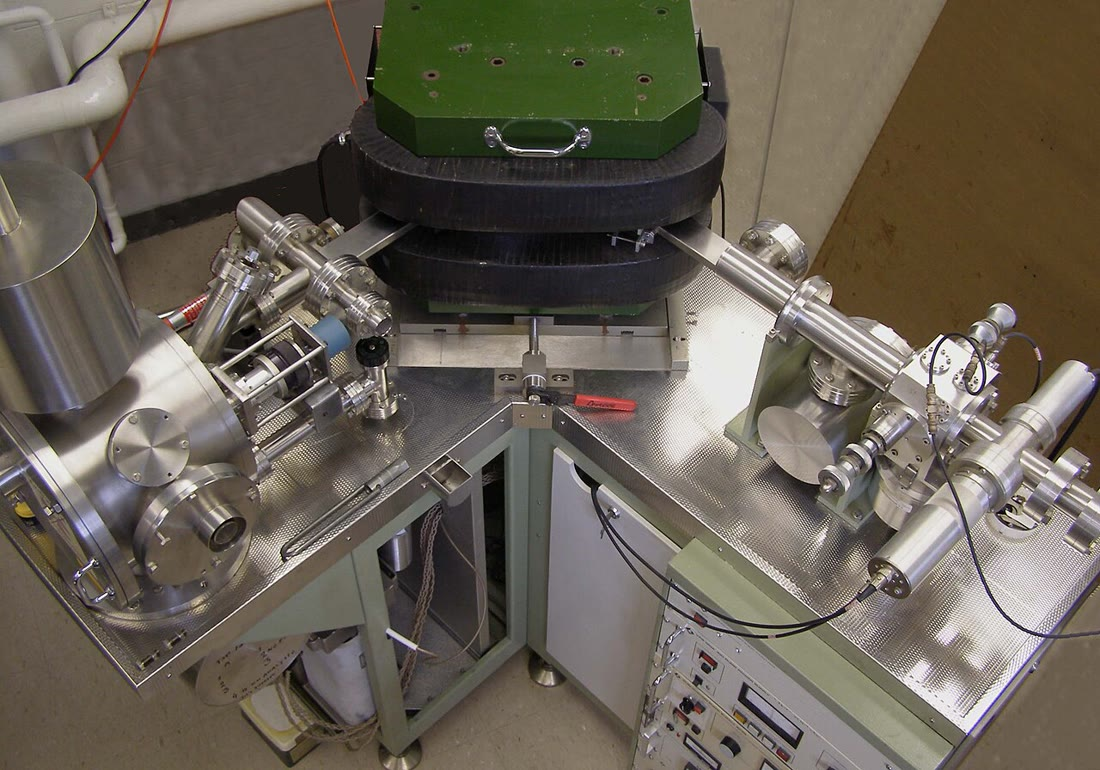
\includegraphics[width=0.42\linewidth]{images/book3/b1-tims.jpg}\hfill
\begin{minipage}[b]{0.55\linewidth}
A thermal ionisation mass spectrometer (left) measures the isotope ratios of
elements such as strontium. The element, separated from the dissolved sample by
chemistry, is loaded on a metal filament in a vacuum; heated, it gives off ions,
which are accelerated and bent by the field of the large electromagnet (the
black coils at the centre), lighter ions more than heavier ones, so that each
isotope reaches its own collector. Ratios of isotopes are what the instrument
measures best, which is why methods built on ratios alone are the most precise.
(Photograph: Radiogenic, CC0, via Wikimedia Commons.)
\end{minipage}
\end{inthelab}
% ledger: commons:tims, amherst:constants

\section{Potassium--argon, uranium--lead and radiocarbon}\label{sec:b1:radiometric-methods:kar}

\subsection*{A parent with two daughters}

\begin{definition}[Branching decay]\label{def:b1:radiometric-methods:branching}
A parent undergoes \emph{branching decay}\index{branching decay} when its nuclei
decay by two or more routes to different daughters. Each route $i$ has its own
partial decay constant $\lambda_i$; the parent decays with the total constant
$\lambda = \sum_i \lambda_i$, and a fraction $\lambda_i/\lambda$ of the decays
take route~$i$. Potassium-40 decays to calcium-40 with $\lambda_\beta =
\num{4.962e-10}$ per year and to argon-40 with $\lambda_e = \num{0.581e-10}$ per
year.
\end{definition}
% ledger: amherst:constants, iaea:k40-branches

\begin{proposition}[The potassium--argon age]\label{prop:b1:radiometric-methods:kar}
A \omterm{def:b1:rock-forming-minerals:mineral}{mineral} that has kept all the argon made in it, and contained none when it
formed, contains after a time $t$
\[
  {}^{40}\mathrm{Ar}^* = \frac{\lambda_e}{\lambda}\;{}^{40}\mathrm{K}\,\bigl(e^{\lambda t} - 1\bigr),
  \qquad\text{so}\qquad
  t = \frac{1}{\lambda}\,\ln\!\left(1 + \frac{\lambda}{\lambda_e}\,
      \frac{{}^{40}\mathrm{Ar}^*}{{}^{40}\mathrm{K}}\right),
\]
where ${}^{40}\mathrm{K}$ is the number of potassium-40 atoms today and $\lambda =
\lambda_\beta + \lambda_e$.
\end{proposition}

\begin{proof}
The parent decays with the total constant $\lambda$, whatever the route, so by
\cref{prop:b1:radiometric-methods:growth} the number of decays in the time $t$ is
${}^{40}\mathrm{K}\,(e^{\lambda t} - 1)$. Each decay takes the argon route with
probability $\lambda_e/\lambda$, independently of the others; over the very
large number of decays the fraction that gave argon is $\lambda_e/\lambda$. This
gives ${}^{40}\mathrm{Ar}^*$; solving for $t$ gives the age.
\end{proof}

The exponent holds the total constant and the factor in front the partial one:
using $\lambda_e$ in the exponent, as if argon were the only route, would give
an age wildly wrong. The calcium branch carries nine-tenths of the decays but is
useless for dating, because calcium-40 is the common isotope of an element
abundant in rocks; argon, a noble gas, escapes from a melt, so that a crystal
starts with almost none. Potassium-40 is \qty{0.0117}{\percent} of the atoms of
potassium. The method needs the absolute amounts of both potassium and argon,
measured separately. Argon from the air, present in every rock, is recognised by
its argon-36 and subtracted with the atmospheric ratio
$^{40}\mathrm{Ar}/^{36}\mathrm{Ar} = 295.5$.
% ledger: tulane:kar, iaea:k40-branches, amherst:constants, nmgrl:kar

The method fails in two ways. Excess argon makes ages too old: a lava that
cools quickly can trap argon from the \omterm{def:b1:layered-earth:layers}{mantle} in bubbles, and historic lavas
usually give potassium--argon ages of 1 to 2 million years, an error that
matters only for young rocks. Argon loss makes them too young: most \omterm{def:b1:rock-forming-minerals:mineral}{minerals}
lose argon when heated above about \qty{300}{\celsius}, so that a later
metamorphism resets the clock wholly or in part, and a partial loss gives an age
between the two events that dates neither. Potassium-rich \omterm{def:b1:rock-forming-minerals:mineral}{minerals} are
preferred: sanidine and biotite, then \omterm{def:b1:rock-forming-minerals:groups}{plagioclase} or hornblende.
% ledger: tulane:kar, nmgrl:kar

The argon--argon method measures only ratios. The sample is irradiated with
fast neutrons in the core of a nuclear reactor, beside a standard \omterm{def:b1:rock-forming-minerals:mineral}{mineral} of
known age; the reaction turns part of its potassium-39 into argon-39, which then
stands for the potassium, and the standard gives the yield of the reaction. The
two isotopes are measured together in the same gas. The sample can then be
heated in steps, with a furnace or a laser; each step gives an age, and the
ages are plotted against the cumulative fraction of argon-39 released, an age
spectrum. Steps that agree within their errors form a plateau; a spectrum
without one warns that the \omterm{def:b1:rock-forming-minerals:mineral}{mineral} has not stayed closed. The synchrony of the
impact and the extinction at the end of the Cretaceous rests on argon--argon
ages.
% ledger: amherst:arar, nmgrl:arar, renne:kpg

\subsection*{Two uranium clocks}

Uranium has two long-lived isotopes, uranium-238 decaying to lead-206 and
uranium-235 to lead-207, at different rates; today
$^{235}\mathrm{U}/^{238}\mathrm{U} = 0.0072567$, one atom in 137.8. A \omterm{def:b1:rock-forming-minerals:mineral}{mineral}
holding uranium thus carries two independent clocks, each with its own
growth equation, ${}^{206}\mathrm{Pb}^* = {}^{238}\mathrm{U}\,(e^{\lambda_{238} t} - 1)$
and ${}^{207}\mathrm{Pb}^* = {}^{235}\mathrm{U}\,(e^{\lambda_{235} t} - 1)$. If the
two ages agree, they are said to be concordant, and the agreement is a test
that the \omterm{def:b1:rock-forming-minerals:mineral}{mineral} stayed closed, which no single clock can provide. Disagreement
comes mostly from lead lost from parts of the crystal damaged by the radiation
of the uranium itself; a graph of the two ratios against each other, the
concordia diagram, then recovers both the age of the crystal and that of the
event that made it lose lead --- a tool of the Year~3 volume.
% ledger: amherst:constants, tulane:upb-zircon

Zircon, $\mathrm{ZrSiO_4}$, is the \omterm{def:b1:rock-forming-minerals:mineral}{mineral} of choice: it takes uranium into its
structure but almost no lead, so that nearly all its lead is radiogenic; it is
hard, resists weathering and survives metamorphism, so that grains eroded from
a rock keep its age in the sands derived from it. Apatite and sphene are used
too, less often.
% ledger: tulane:upb-zircon, commons:zircon-cl

\subsection*{Radiocarbon}

Carbon-14 is made continually in the upper atmosphere from nitrogen-14 struck
by cosmic rays. It joins the carbon of the atmosphere; living organisms
exchange carbon with the atmosphere and keep its proportion of carbon-14. At
death the exchange stops and the carbon-14 decays back to nitrogen-14. Since the
initial proportion is that of the atmosphere, the age follows from the decay
law alone, without an \omterm{def:b1:radiometric-methods:isochron}{isochron}: $t = -\tau \ln(A/A_0)$, where $A$ is the
activity of the sample's carbon, $A_0$ that of living carbon and $\tau =
1/\lambda$ the mean life. Wood, charcoal, bone, teeth and shell are dated this
way, up to some tens of thousands of years: about \num{70000} years at most.
% ledger: tulane:c14, iaea:c14

\begin{definition}[Radiocarbon age, calibration curve]\label{def:b1:radiometric-methods:radiocarbon}
The (conventional) \emph{radiocarbon age}\index{radiocarbon age} of a sample is
\[
  t = -8033 \,\ln \frac{A_{\mathrm{SN}}}{A_{\mathrm{ON}}} \ \text{years BP},
\]
where $A_{\mathrm{SN}}$ is the activity of the sample's carbon and
$A_{\mathrm{ON}}$ that of the reference standard; it uses the half-life of
\num{5568} years (mean life \num{8033} years), normalises the activities for
the isotopic fractionation of carbon ($\delta^{13}\mathrm{C} = \qty{-25}{\permil}$),
and counts years before AD~1950 (BP, ``before present''). A
\emph{calibration curve}\index{calibration curve} gives the radiocarbon age of
samples of known calendar age; read backwards, it converts a radiocarbon age into
a range of calendar ages (cal BP).
\end{definition}
% ledger: sp77:conventional-age, reimer20:intcal20

The \omterm{def:b1:radiometric-methods:radiocarbon}{radiocarbon age} is not an age in calendar years, for two reasons. The
half-life of \num{5568} years, Libby's value, kept by convention, is shorter than the true \num{5700} years, so \omterm{def:b1:radiometric-methods:radiocarbon}{radiocarbon ages} run about
\qty{2.4}{\percent} short. More importantly, the proportion of carbon-14 in the
atmosphere has not been constant. The \omterm{def:b1:radiometric-methods:radiocarbon}{calibration curve} measures both effects
together, on archives dated independently: tree rings back to about
\num{13900} cal BP, and beyond, floating tree-ring sequences, lake and
marine sediments, cave deposits and corals, to \num{55000} cal BP (figure below).
% ledger: sp77:conventional-age, iaea:c14, reimer20:intcal20

\begin{omfigure}
\begin{tikzpicture}
\begin{axis}[name=main, omrecord, width=0.5\linewidth, height=6cm, xmin=0, xmax=12, ymin=0, ymax=12,
  xlabel={calendar age (thousand cal BP)}, ylabel={radiocarbon age (thousand BP)},
  xtick={0,2,...,12}, ytick={0,2,...,12}]
% figdata/bachelor-1/radiocarbon.py, IntCal20 (dataset bachelor-1-intcal20); ledger: data:b3-intcal20
\addplot[black!50, dashed, domain=0:12, samples=2] {x};
\addplot[omDef, line width=0.9pt] table[x=cal, y=c14] {figdata/out/bachelor-1-radiocarbon-curve.dat};
\draw[omThm, line width=0.6pt] (axis cs:2.3,2.3) rectangle (axis cs:2.9,2.9);
\node[font=\scriptsize, anchor=east, text=black!60] at (axis cs:8.4,10.4) {equal ages};
\node[font=\scriptsize, text=omDef, anchor=north west] at (axis cs:7.4,5.6) {IntCal20};
\end{axis}
\begin{axis}[at={(main.east)}, anchor=west, xshift=2.1cm, omrecord, width=0.38\linewidth, height=6cm,
  xmin=2300, xmax=2900, ymin=2300, ymax=2900, xlabel={calendar age (cal BP)}, ylabel={radiocarbon age (BP)},
  xtick={2300,2500,2700,2900}, ytick={2300,2500,2700,2900},
  x tick label style={/pgf/number format/.cd, set thousands separator={}},
  y tick label style={/pgf/number format/.cd, set thousands separator={}}]
\addplot[name path=hi, draw=none, forget plot] table[x=cal, y=hi] {figdata/out/bachelor-1-radiocarbon-zoom.dat};
\addplot[name path=lo, draw=none, forget plot] table[x=cal, y=lo] {figdata/out/bachelor-1-radiocarbon-zoom.dat};
\addplot[omDef!25, forget plot] fill between[of=hi and lo];
\addplot[omDef, line width=0.8pt] table[x=cal, y=c14] {figdata/out/bachelor-1-radiocarbon-zoom.dat};
\addplot[omThm, line width=0.6pt, domain=2300:2900, samples=2] {2480};
\draw[omThm, densely dotted] (axis cs:2495,2300) -- (axis cs:2495,2480);
\draw[omThm, densely dotted] (axis cs:2699,2300) -- (axis cs:2699,2480);
\node[font=\scriptsize, text=omThm, anchor=south west] at (axis cs:2310,2485) {$2480$ BP};
\end{axis}
\end{tikzpicture}

{\small Left: the IntCal20 \omterm{def:b1:radiometric-methods:radiocarbon}{calibration curve} over the last \num{12000} years,
\omterm{def:b1:radiometric-methods:radiocarbon}{radiocarbon age} against calendar age; the dashed line is where the two would be
equal. Right: the box on the left enlarged, with the band of one standard
uncertainty of the curve. Between \num{2500} and \num{2700} cal BP the curve
is nearly flat: a \omterm{def:b1:radiometric-methods:radiocarbon}{radiocarbon age} of 2480 years BP matches calendar ages
from about \num{2495} to \num{2699} cal BP.}
\label{fig:b1:radiometric-methods:intcal}
\end{omfigure}
% ledger: data:b3-intcal20, reimer20:intcal20

At \num{2000} cal BP the curve gives \num[uncertainty-mode=separate]{2070 \pm 14} years BP; at
\num{12000} cal BP, \num{10306}: \omterm{def:b1:radiometric-methods:radiocarbon}{radiocarbon ages} there are \num{1694} years
younger than calendar ages, far more than the \qty{2.4}{\percent} of the
half-life. The curve wiggles, and where it is flat a \omterm{def:b1:radiometric-methods:radiocarbon}{radiocarbon age} matches a
long range of calendar ages, however precise the measurement.
% ledger: data:b3-intcal20

\begin{dated}{2020}
% ledger: reimer20:intcal20
The curve in use for the Northern Hemisphere is IntCal20, published in 2020. It
replaced IntCal13, adding new data and extending the curve to \num{55000} cal BP,
with separate curves for the Southern Hemisphere and for the surface ocean.
\omterm{def:b1:radiometric-methods:radiocarbon}{Calibration curves} are revised as new archives are measured, so a calendar age
must name the curve that produced it.
\end{dated}

\section{Closure temperature}\label{sec:b1:radiometric-methods:closure}

A \omterm{def:b1:rock-forming-minerals:mineral}{mineral} that crystallises from a magma at \qty{800}{\celsius} does not start
its clock at once. While it is hot, atoms of the daughter --- argon above all ---
diffuse through its lattice and escape; only when it has cooled enough does
diffusion become too slow to matter, and the daughter begin to accumulate.
% ledger: leeds:closure, tulane:kar, tulane:magma-types

\begin{definition}[Closure temperature, cooling age]\label{def:b1:radiometric-methods:closure}
The \emph{closure temperature}\index{closure temperature} of a \omterm{def:b1:rock-forming-minerals:mineral}{mineral} for a
decay system is the temperature below which the parent and daughter atoms no
longer diffuse in or out of its lattice fast enough to matter, so that the
\omterm{def:b1:rock-forming-minerals:mineral}{mineral} behaves as a closed system. A \emph{cooling age}\index{cooling age} is an
age measured in a \omterm{def:b1:rock-forming-minerals:mineral}{mineral} that formed above its closure temperature: it dates
the moment the \omterm{def:b1:rock-forming-minerals:mineral}{mineral} cooled through that temperature, not the moment it
formed.
\end{definition}
% ledger: leeds:closure

\omterm{def:b1:radiometric-methods:closure}{Closure temperatures} differ by \omterm{def:b1:rock-forming-minerals:mineral}{mineral}, because the lattices differ, and by
element, because different atoms diffuse through one lattice at different rates
(figure below). They are approximate: two tables give \qty{280}{\celsius} and
\qty{350}{\celsius} for argon in biotite, \qty{530}{\celsius} and
\qty{550}{\celsius} for argon in hornblende. Fission tracks, the trails of damage
left in a crystal by the spontaneous fission of uranium nuclei, heal at even lower
temperatures.
% ledger: leeds:closure, amherst:closure

\begin{omfigure}
\begin{tikzpicture}
\begin{axis}[width=0.8\linewidth, height=7cm, xbar, bar width=7pt, xmin=0, xmax=850,
  xlabel={closure temperature (\unit{\celsius})},
  symbolic y coords={zrupb,spupb,hbar,mssr,msar,btsr,btar,zrft,kfsar,apft},
  ytick={zrupb,spupb,hbar,mssr,msar,btsr,btar,zrft,kfsar,apft}, y dir=reverse, enlarge y limits=0.07,
  yticklabels={{zircon, U--Pb},{sphene, U--Pb},{hornblende, K--Ar},{muscovite, Rb--Sr},{muscovite, K--Ar},{biotite, Rb--Sr},{biotite, K--Ar},{zircon, fission tracks},{K-feldspar, K--Ar},{apatite, fission tracks}},
  y tick label style={font=\scriptsize}, x tick label style={font=\scriptsize},
  axis x line*=bottom, axis y line*=left]
% ledger: leeds:closure (values as tabulated; > lower bound, ~ approximate, ranges and +- as given)
\addplot[fill=omDef!55, draw=omDef, error bars/.cd, x dir=both, x explicit]
  coordinates {(750,zrupb) (650,spupb) (530,hbar) +- (40,0) (500,mssr) (350,msar) (320,btsr)
               (280,btar) +- (40,0) (200,zrft) +- (25,0) (130,kfsar) (105,apft) +- (10,0)};
\node[font=\scriptsize, anchor=west] at (axis cs:755,zrupb) {$> 750$};
\node[font=\scriptsize, anchor=west] at (axis cs:655,spupb) {$> 650$};
\node[font=\scriptsize, anchor=west] at (axis cs:575,hbar) {$530 \pm 40$};
\node[font=\scriptsize, anchor=west] at (axis cs:505,mssr) {$500$};
\node[font=\scriptsize, anchor=west] at (axis cs:355,msar) {$\approx 350$};
\node[font=\scriptsize, anchor=west] at (axis cs:325,btsr) {$320$};
\node[font=\scriptsize, anchor=west] at (axis cs:325,btar) {$280 \pm 40$};
\node[font=\scriptsize, anchor=west] at (axis cs:230,zrft) {$175$--$225$};
\node[font=\scriptsize, anchor=west] at (axis cs:135,kfsar) {$\approx 130$, leaky};
\node[font=\scriptsize, anchor=west] at (axis cs:120,apft) {$105 \pm 10$};
\end{axis}
\end{tikzpicture}

{\small \omterm{def:b1:radiometric-methods:closure}{Closure temperatures} of the main \omterm{def:b1:rock-forming-minerals:mineral}{mineral} clocks, from one published table.
U--Pb is uranium--lead, K--Ar potassium--argon (and argon--argon), Rb--Sr
rubidium--strontium. For fission tracks the value is the temperature at which the
tracks heal.}
\label{fig:b1:radiometric-methods:closure}
\end{omfigure}

In a pluton that cooled slowly, the clocks therefore close one after another,
from the hottest to the coolest: zircon first, near its crystallisation, then
hornblende, then muscovite and biotite. The spread of their ages records the
cooling.

\begin{proposition}[Cooling rate between two closures]\label{prop:b1:radiometric-methods:cooling}
If two \omterm{def:b1:rock-forming-minerals:mineral}{minerals} of one rock, of \omterm{def:b1:radiometric-methods:closure}{closure temperatures} $T_1 > T_2$, give the \omterm{def:b1:radiometric-methods:closure}{cooling
ages} $t_1 > t_2$, the mean cooling rate between the two closures is
\[
  \dot T = \frac{T_1 - T_2}{t_1 - t_2}.
\]
If the rock lay at a depth where the temperature rose with depth at a constant
gradient $G$ below a surface at the temperature $T_s$, it was at the depth $z_i
= (T_i - T_s)/G$ when the clock $i$ closed.
\end{proposition}

\begin{proof}
The rock was at $T_1$ at the time $t_1$ and at $T_2$ at the time $t_2$; the mean
rate of change of its temperature is the ratio of the two differences. With a
linear \omterm{def:b1:heat-budget:geotherm}{geotherm} (\cref{def:b1:heat-budget:geotherm}), $T = T_s + G z$, which
gives the depth.
\end{proof}

The depth gives a rate of exhumation once the time the rock reached the surface
is known --- as in the problem of this chapter. The method is crude: the
\omterm{def:b1:radiometric-methods:closure}{closure temperatures} are uncertain by tens of degrees, and the \omterm{def:b1:heat-budget:geotherm}{geotherm} is
assumed constant through time. Thermochronology, the
detailed reconstruction of temperature--time paths from many clocks, is a subject
of the Year~3 volume.

\section{Dating sedimentary sequences}\label{sec:b1:radiometric-methods:sediments}

Most sedimentary rocks cannot be dated directly. Their grains are older than the
rock: a detrital zircon, like the grain at the head of this chapter, dates the
rock it was eroded from. Radiocarbon dates only young organic matter. The ages
of the chart therefore come from rocks that crystallised at the moment they
were deposited --- volcanic ash and lava flows within the sequence --- and from
igneous rocks that cut it.
% ledger: tulane:upb-zircon, tulane:c14, commons:zircon-cl

\begin{definition}[Bracketing age]\label{def:b1:radiometric-methods:bracketing}
A \emph{bracketing age}\index{bracketing age} is a limit placed on the age of a
sedimentary level by dated rocks related to it by the principles of
stratigraphy: a maximum age from a dated layer below it, or from the youngest
detrital grain in it; a minimum age from a dated layer above it, or from an
intrusion that cuts it. A level between a maximum and a minimum is bracketed.
\end{definition}

\begin{omfigure}
\begin{tikzpicture}[x=1cm, y=0.62cm]
  % column
  \fill[lith shale] (0,0) rectangle (2.4,3);
  \fill[lith sandstone] (0,3) rectangle (2.4,6);
  \fill[lith shale] (0,6) rectangle (2.4,9);
  \fill[lith limestone] (0,9) rectangle (2.4,12);
  \draw (0,0) rectangle (2.4,12);
  % ash bed below, lava flow above
  \fill[omThm!70] (0,2.0) rectangle (2.4,2.3);
  \fill[black!65] (0,9.0) rectangle (2.4,9.6);
  % boundary
  \draw[omDef, line width=1.2pt] (-0.3,7.2) -- (2.7,7.2);
  % dyke cutting everything
  \fill[black!40] (1.55,0) -- (1.85,0) -- (1.95,12) -- (1.65,12) -- cycle;
  % detrital zircons
  \foreach \p in {(0.4,3.6),(0.9,4.5),(0.5,5.4),(1.2,3.9),(0.8,5.0)}
    \fill[omThm] \p circle (1.3pt);
  % labels
  \node[anchor=west, font=\small, align=left] at (3.0,2.15) {ash bed, $t_1$: maximum age};
  \node[anchor=west, font=\small, align=left] at (3.0,4.5) {youngest detrital zircon, $t_0$:\\maximum age of the sandstone};
  \node[anchor=west, font=\small, text=omDef] at (3.0,7.2) {level to be dated};
  \node[anchor=west, font=\small, align=left] at (3.0,9.3) {lava flow, $t_2$: minimum age};
  \node[anchor=west, font=\small, align=left] at (3.0,11.3) {dyke, $t_3$: minimum age of\\every layer it cuts};
  \draw[black!50] (2.5,2.15) -- (2.95,2.15);
  \draw[black!50] (1.25,4.5) -- (2.95,4.5);
  \draw[black!50] (2.5,9.3) -- (2.95,9.3);
  \draw[black!50] (1.95,11.3) -- (2.95,11.3);
\end{tikzpicture}

{\small Ages that bracket a level in a sedimentary sequence (schematic). The
ash bed below and the youngest detrital zircon in the sandstone give maximum ages;
the lava flow above and the dyke that cuts the whole sequence give minimum ages.
The level is younger than $t_1$ and older than $t_2$; the dyke adds only that it
is older than $t_3$.}
\label{fig:b1:radiometric-methods:bracketing}
\end{omfigure}

The best brackets are close and precise: two ash beds a few metres apart, dated
on zircon to a few tens of thousands of years, with the level between them
interpolated by \cref{prop:b1:stratigraphic-scale:interpolation}. At Meishan,
the GSSP of the base of the Triassic lies among five dated ash beds; the
extinction is bracketed between \qty[uncertainty-mode=separate]{251.941(37)}{\Ma}
and \qty[uncertainty-mode=separate]{251.880(31)}{\Ma}, and the base of the system
is placed at \qty[uncertainty-mode=separate]{251.902(24)}{\Ma}
(\cref{sec:b1:stratigraphic-scale:extinctions}). Ash beds, carried by the wind
across facies, are both time lines and clocks.
% ledger: burgess:end-permian, gssp:induan, ics:base.Triassic

The chart is only as precise as the dated beds near each boundary. The base of
the Triassic is known to \qty{0.024}{\Myr}, one part in ten thousand; the base of
the Carboniferous to \qty{0.19}{\Myr}; the base of the Devonian to
\qty{1.36}{\Myr}. Where no dated bed lies near a boundary, its age is
interpolated between distant ones, and its uncertainty grows accordingly. Each
new ash bed dated near a boundary can move it, which is why the chart carries a
version date.
% ledger: ics:base.Triassic, ics:base.Carboniferous, gssp:lochkovian

\section{Exercises}

\begin{exercise}[$\star$]\label{exo:b1:radiometric-methods:1}
(a)~A \omterm{def:b1:rock-forming-minerals:mineral}{mineral} contains three times as many \omterm{def:b1:radiometric-methods:radiogenic}{radiogenic daughter} atoms as parent
atoms. How many half-lives old is it? (b)~Compute $D^*/P$ after
\qty{310}{\Myr} for rubidium-87 and for uranium-235, with the constants of
\cref{tab:b1:radiometric-methods:systems}. Which ratio is easier to measure
precisely? (c)~After how many half-lives is less than \qty{1}{\percent} of the
parent left?
% ledger: villa22:rb87, amherst:constants
\end{exercise}

\begin{exercise}[$\star$]\label{exo:b1:radiometric-methods:2}
Which method of \cref{tab:b1:radiometric-methods:systems} would you use, and on
what material, to date: (a)~charcoal from a hearth about \num{8000} years old;
(b)~an ash bed thought to be about \qty{66}{\Ma} old, rich in sanidine and
zircon; (c)~a granite about \qty{2.7}{\Ga} old; (d)~a shell about
\num{40000} years old; (e)~a limestone of the Jurassic with no volcanic layer?
% ledger: tulane:c14, tulane:kar, tulane:upb-zircon
\end{exercise}

\begin{exercise}[$\star$]\label{exo:b1:radiometric-methods:3}
The carbon of a piece of wood has a quarter of the activity of the standard,
after normalisation. (a)~Compute its conventional \omterm{def:b1:radiometric-methods:radiocarbon}{radiocarbon age}. (b)~Compute
its age with the half-life of \num{5700} years. (c)~Why is neither of these its
age in calendar years, and how is that age obtained?
% ledger: sp77:conventional-age, iaea:c14
\end{exercise}

\begin{exercise}[$\star$]\label{exo:b1:radiometric-methods:4}
A granite gives a uranium--lead age on zircon of \qty{420}{\Ma}, a
potassium--argon age on hornblende of \qty{410}{\Ma} and one on biotite of
\qty{398}{\Ma}. (a)~Why are the three ages different, and in this order?
(b)~With the \omterm{def:b1:radiometric-methods:closure}{closure temperatures} of the figure of
\cref{sec:b1:radiometric-methods:closure}, compute the mean cooling rate between
the closures of hornblende and biotite. (c)~What can be said of the cooling rate
between the closure of zircon and that of hornblende?
% ledger: leeds:closure
\end{exercise}

\begin{exercise}[$\star\star$]\label{exo:b1:radiometric-methods:5}
Four whole-rock samples of a gneiss (exercise data) give
$^{87}\mathrm{Rb}/^{86}\mathrm{Sr} = 2.0$, $5.0$, $9.0$, $14.0$ and
$^{87}\mathrm{Sr}/^{86}\mathrm{Sr} = 0.7323$, $0.7741$, $0.8307$, $0.9010$.
(a)~Fit the least-squares line by the method of
\cref{met:b1:radiometric-methods:isochron}. (b)~Compute the age and the \omterm{def:b1:radiometric-methods:isochron}{initial
ratio}. (c)~Compute $s$ and the uncertainty of the age. (d)~Does the \omterm{def:b1:radiometric-methods:isochron}{initial ratio}
point to a source in the \omterm{def:b1:layered-earth:layers}{mantle} or in the \omterm{def:b1:layered-earth:layers}{crust}?
% ledger: villa22:rb87, tulane:sr-initial
\end{exercise}

\begin{exercise}[$\star\star$]\label{exo:b1:radiometric-methods:6}
A sanidine from an ash bed contains \qty{10.0}{\percent} potassium by mass and
\qty{1.169}{nmol} of radiogenic argon-40 per gram. (a)~With the atomic weight of
potassium, \qty{39.098}{g.mol^{-1}}, and the abundance of potassium-40, compute
the number of moles of potassium-40 per gram. (b)~Compute the potassium--argon
age. (c)~If \qty{0.5}{\percent} of the argon measured had been trapped when the
ash fell rather than made by decay, by how much would the age be too old? Is this
a concern here?
% ledger: ciaaw:K, iaea:k40-branches, amherst:constants, tulane:kar
\end{exercise}

\begin{exercise}[$\star\star$]\label{exo:b1:radiometric-methods:7}
The IntCal20 curve gives the \omterm{def:b1:radiometric-methods:radiocarbon}{radiocarbon ages} \num[uncertainty-mode=separate]{2070 \pm 14} years BP at \num{2000}
cal BP, \num{7178} at \num{8000} cal BP and \num{10306} at \num{12000} cal BP.
(a)~A seed gives \num[uncertainty-mode=separate]{2070 \pm 14} years BP. What is its
calendar age? (b)~Another gives \num[uncertainty-mode=separate]{2480 \pm 15} years
BP; with the right-hand panel of the figure of
\cref{sec:b1:radiometric-methods:kar}, give its range of calendar ages and explain
why it is so wide. (c)~By how many years, and in which direction, do \omterm{def:b1:radiometric-methods:radiocarbon}{radiocarbon
ages} differ from calendar ages at \num{2000}, \num{8000} and \num{12000} cal BP?
Does the difference grow in proportion to the age?
% ledger: data:b3-intcal20
\end{exercise}

\begin{exercise}[$\star\star$]\label{exo:b1:radiometric-methods:8}
In a marine section, an ash bed at \qty{4}{m} is dated
\qty[uncertainty-mode=separate]{94.50(10)}{\Ma} and a lava flow at \qty{20}{m}
\qty[uncertainty-mode=separate]{93.80(12)}{\Ma}; a dyke that cuts the whole
section is dated \qty[uncertainty-mode=separate]{93.20(8)}{\Ma}. The youngest
detrital zircon in a sandstone at \qtyrange{6}{10}{m} is
\qty[uncertainty-mode=separate]{95.3(4)}{\Ma}. A stage boundary is placed at
\qty{12}{m}. (a)~Which of the four ages bracket the boundary, and which are of no
use for it? (b)~Interpolate its age and its uncertainty with
\cref{prop:b1:stratigraphic-scale:interpolation}. (c)~What does the detrital
zircon tell about the sandstone?
\end{exercise}

\begin{exercise}[$\star\star$]\label{exo:b1:radiometric-methods:9}
Two zircons of one granite give
$^{206}\mathrm{Pb}^*/^{238}\mathrm{U} = 0.08401$ and
$^{207}\mathrm{Pb}^*/^{235}\mathrm{U} = 0.6688$ (grain~A), and $0.05881$ and
$0.4682$ (grain~B). (a)~Compute the two ages of each grain. (b)~Which grain is
concordant? (c)~Grain~B has lost part of its lead recently. Show that both its
ratios are \qty{70}{\percent} of those of grain~A, and explain why its two ages
differ although the loss was the same for both isotopes.
% ledger: amherst:constants, tulane:upb-zircon
\end{exercise}

\begin{exercise}[$\star\star\star$]\label{exo:b1:radiometric-methods:10}
(a)~Show that when $\lambda t \ll 1$ the age equation reduces to $t \approx
(D^*/P)/\lambda$, and that the relative error of this approximation is close to
$\lambda t/2$. (b)~Compute the error for rubidium-87 at \qty{310}{\Ma}, for
potassium-40 at \qty{296}{\Ma} and for uranium-238 at \qty{4.4}{\Ga}. (c)~If
$D^*/P$ is measured to \qty{0.1}{\percent}, what is the uncertainty of a
rubidium--strontium age of \qty{310}{\Ma}?
% ledger: villa22:rb87, amherst:constants
\end{exercise}

\begin{exercise}[$\star\star\star$]\label{exo:b1:radiometric-methods:11}
A biotite crystallised and closed \qty{400}{\Myr} ago. \qty{200}{\Myr} ago a
brief heating made it lose a fraction $f$ of its argon, after which it was closed
again. (a)~Show that today
\[
  \frac{\lambda}{\lambda_e}\,\frac{^{40}\mathrm{Ar}^*}{^{40}\mathrm{K}} =
  (1 - f)\bigl(e^{\lambda t_1} - e^{\lambda t_2}\bigr) + e^{\lambda t_2} - 1,
\]
with $t_1 = \qty{400}{\Myr}$ and $t_2 = \qty{200}{\Myr}$. (b)~Compute the
apparent potassium--argon age for $f = 0$, $0.3$, $0.6$ and $1$. (c)~Why can a
single potassium--argon age not tell a partial loss from a younger event?
% ledger: amherst:constants, tulane:kar
\end{exercise}

\begin{exercise}[$\star\star\star$]\label{exo:b1:radiometric-methods:12}
At \num{12000} cal BP the IntCal20 curve gives a \omterm{def:b1:radiometric-methods:radiocarbon}{radiocarbon age} of
\num{10306} years BP. (a)~Recompute the age from the same activity ratio with the
half-life of \num{5700} years. (b)~How much of the \num{1694} years by which the
\omterm{def:b1:radiometric-methods:radiocarbon}{radiocarbon age} falls short of the calendar age does the half-life convention
explain? (c)~Assuming the rest comes from a higher proportion of carbon-14 in the
atmosphere \num{12000} years ago, compute by how much, in per cent, it exceeded
the proportion of the standard.
% ledger: data:b3-intcal20, sp77:conventional-age, iaea:c14
\end{exercise}

\section{Problem: Dating the Varden granite and its cover}

\begin{problem}[{Weekend problem --- how four clocks date the crystallisation,
the cooling and the unroofing of a granite}]
\label{pb:b1:radiometric-methods:1}
% values: calc/ch25.py; the analyses are invented, consistent with the Varden granite of 310 Ma (region.py)
The granite of the Varden Hills, the series' invented region, intrudes the
schist basement and is overlain, above an \omterm{def:b1:cross-sections:unconformity}{unconformity}, by the Triassic
sandstone. Use the constants of \cref{tab:b1:radiometric-methods:systems}, the
\omterm{def:b1:radiometric-methods:closure}{closure temperatures} of the figure of \cref{sec:b1:radiometric-methods:closure},
the atomic weight of potassium \qty{39.098}{g.mol^{-1}} and the abundance of
potassium-40, \qty{0.0117}{\percent} of the atoms of potassium. All analyses are
exercise data.

\medskip
\noindent\textbf{Part I --- A whole-rock isochron.} Six whole-rock samples give:
\begin{center}
\small
\begin{tabular}{|l|cccccc|}
\hline
$^{87}\mathrm{Rb}/^{86}\mathrm{Sr}$ & 0.92 & 2.15 & 3.40 & 5.05 & 7.60 & 10.30 \\
$^{87}\mathrm{Sr}/^{86}\mathrm{Sr}$ & 0.71211 & 0.71718 & 0.72284 & 0.72986 & 0.74113 & 0.75261 \\
\hline
\end{tabular}
\end{center}
\begin{enumerate}
  \item Plot the six samples. Do they lie on a straight line?
  \item Compute $\bar x$, $\bar y$, $S_{xx}$ and $S_{xy}$, then the
        least-squares slope.
  \item Compute the intercept. What does it represent?
  \item Compute the age of the granite.
  \item Compute the residuals, $s$, and the uncertainty of the age.
  \item Is the \omterm{def:b1:radiometric-methods:isochron}{initial ratio} closer to that of the \omterm{def:b1:layered-earth:layers}{mantle} or of the continental
        \omterm{def:b1:layered-earth:layers}{crust}? If the magma were a mixture of melts with $0.7025$ and $0.710$,
        equally rich in strontium, what share of its strontium came from the
        \omterm{def:b1:layered-earth:layers}{crust}?
\end{enumerate}

\noindent\textbf{Part II --- Potassium and argon.} A biotite contains
\qty{7.40}{\percent} potassium by mass and \qty{4.139}{nmol} of radiogenic
argon-40 per gram; a hornblende \qty{1.10}{\percent} and \qty{0.6333}{nmol.g^{-1}}.
\begin{enumerate}[resume]
  \item Compute the number of atoms of potassium-40 in a gram of the biotite.
  \item Compute the potassium--argon age of the biotite.
  \item Compute that of the hornblende.
  \item What age would the biotite give if the branching were forgotten and all
        decays counted as argon? Why is calcium-40 not used instead?
  \item Why is excess argon, trapped when the \omterm{def:b1:rock-forming-minerals:mineral}{minerals} formed, of little concern
        here?
  \item Both ages are younger than the \omterm{def:b1:radiometric-methods:isochron}{isochron} age. Give two explanations, and
        say how an argon--argon age spectrum could tell them apart.
\end{enumerate}

\noindent\textbf{Part III --- Cooling.} A zircon of the granite gives
$^{206}\mathrm{Pb}^*/^{238}\mathrm{U} = 0.049361$ and
$^{207}\mathrm{Pb}^*/^{235}\mathrm{U} = 0.35784$.
\begin{enumerate}[resume]
  \item Compute the two uranium--lead ages. Are they concordant?
  \item Assign to each age of Parts I to III the event it dates. Draw the
        temperature of the granite against time from the zircon to the biotite.
  \item Compute the mean cooling rate between the closures of hornblende and
        biotite.
  \item What can be said of the cooling rate between the closure of the zircon
        and that of the hornblende?
  \item With an uncertainty of \qty{40}{\celsius} on each of the two \omterm{def:b1:radiometric-methods:closure}{closure
        temperatures}, independent, what range of cooling rates is possible?
  \item With the other table quoted in the chapter (\qty{550}{\celsius} for
        hornblende, \qty{350}{\celsius} for biotite), what rate is found? What
        does this say of the result?
  \item Assume a \omterm{def:b1:heat-budget:geotherm}{geotherm} of \qty{30}{\celsius.km^{-1}} below a surface at
        \qty{10}{\celsius}. At what depth was the granite when the biotite
        closed?
\end{enumerate}

\noindent\textbf{Part IV --- The unconformity.} An ash bed \qty{18}{m} above the
base of the Triassic sandstone contains zircons with
$^{206}\mathrm{Pb}^*/^{238}\mathrm{U} = 0.039108$ and
$^{207}\mathrm{Pb}^*/^{235}\mathrm{U} = 0.27577$. A second ash bed, \qty{58}{m}
above the base, is dated \qty{245.30}{\Ma}. Detrital zircons in the lowest metre
of the sandstone give ages around \qty{310}{\Ma}.
\begin{enumerate}[resume]
  \item Compute the age of the lower ash bed.
  \item Where do the detrital zircons come from, and what do they say about the
        age of the sandstone?
  \item Compute the rate of accumulation of the sandstone between the ash beds,
        and the age of its base, assuming the same rate below the lower ash.
  \item How long is the gap in the record at the \omterm{def:b1:cross-sections:unconformity}{unconformity}, from the
        crystallisation of the granite to the deposition of the sandstone?
  \item Compute the mean rate of erosion that brought the granite from the depth
        of question~19 to the surface. What assumption does this make about where
        the eroded granite lay?
  \item What is the cooling rate of the granite?
\end{enumerate}
\end{problem}
